%==============================================================================
% Sjabloon poster bachproef
%==============================================================================
% Gebaseerd op document class `a0poster' door Gerlinde Kettl en Matthias Weiser
% Aangepast voor gebruik aan HOGENT door Jens Buysse en Bert Van Vreckem
\documentclass[a0,portrait]{hogent-poster}
\usepackage{pgfplots} % used for graph generation 

% Info over de opleiding
\course{Bachelorproef}
\studyprogramme{toegepaste informatica}
\academicyear{2023-2024}
\institution{Hogeschool Gent, Valentin Vaerwyckweg 1, 9000 Gent}

% Info over de bachelorproef
\title{Het Web rekent op WebGPU}
\subtitle{Lokale inferentie met WebGPU ondersteunde browsers}
\author{Joris Van Duyse}
\email{joris.vanduyse@student.hogent.be}
\supervisor{Dhr. Thomas Desmedt}
\cosupervisor{Ing. Jonas Welvaert}

% Indien ingevuld, wordt deze informatie toegevoegd aan het einde van de
% abstract. Zet in commentaar als je dit niet wilt.
\specialisation{Enterprise- en Web-development}
\keywords{}
\projectrepo{https://github.com/JorisVanDuyseHogent/Bachelorproef-WebGPU-Ai}

\begin{document}

\maketitle

\begin{abstract}
  De opkomst van kunstmatige intelligentie \textit{(AI)} heeft de vraag naar \textit{server-side} rekenkracht verhoogd. Dit heeft een impact op kosten en het milieu. \textit{WebGPU} als nieuwe browser technologie kan een oplossing bieden voor deze uitdagingen door lokale rekenkracht beschikbaar te stellen. Dit onderzoek beschrijft en test de mogelijkheden van \textit{WebGPU} voor \textit{AI}-toepassingen. \textit{WebGPU} kan inferentie, essentieel voor \textit{AI}-modellen, lokaal uitvoeren, wat serverbelasting vermindert. Dit kan \textit{AI}-toepassingen sneller, gebruiksvriendelijker en goedkoper maken voor zowel gebruikers als bedrijven. Door \textit{WebGPU} te combineren met \textit{large language models}, wordt de prestatie vergeleken met bestaande technologieën, wat de potentie van \textit{WebGPU} voor \textit{AI}-ondersteuning op het web aantoont.
\end{abstract}

\begin{multicols}{2} % This is how many columns your poster will be broken into, a portrait poster is generally split into 2 columns

\section{Introductie}

De lancering van \textit{OpenAI}'s \textit{ChatGPT} bracht een revolutionaire impact, waarvan de schaal moeilijk in te schatten is. \textit{AI}-technologieën, zoals \textit{large language models}, zullen de interactie van eindgebruikers met technologie sterk beïnvloeden. Browsertechnologie maakt \textit{AI} toegankelijker zonder complex installatieproces, maar vereist dat \textit{AI}-modellen operationeel blijven via grote datacentra.

Nieuwe technologieën zoals \textit{Progressive Web Apps} \textit{(PWA's)} vereenvoudigen de installatie van webapplicaties en kunnen kunstmatige intelligentie gebruiksvriendelijker maken. Echter, grootschalige implementatie van \textit{AI} brengt hoge kosten voor \textit{cloudproviders} met zich mee, die uiteindelijk de eindgebruikers betalen. Voor een duurzame en privacybewuste inzet van \textit{AI} moet onderzocht worden hoe deze technologie efficiënt op grote schaal kan worden toegepast, waarbij de kosten en milieueffecten minimaal blijven.

\section{Experimenten}

De prestaties van \textit{WebGPU} voor \textit{embedding} modellen werden getest en vergeleken met \textit{Web Assembly} (\textit{WASM}) op verschillende hardwareconfiguraties binnen de browser. Daarnaast werd de uitvoeringstijd van het \textit{Whisper AI}-model van \textit{OpenAI} vergeleken tussen \textit{CPU}, \textit{CUDA}, en \textit{WebGPU} implementaties op verschillende hardwareconfiguraties en modelgroottes. De testresultaten toonden aan dat \textit{WebGPU} aanzienlijke prestatievoordelen biedt ten opzichte van \textit{CPU}'s, hoewel het nog niet even performant is als \textit{CUDA}. Dit benadrukt de haalbaarheid en efficiëntie van \textit{WebGPU} voor \textit{AI}-inferentie in de browser, met voordelen zoals lokale verwerking en verhoogde privacy voor gebruikers.

Deze testen waren cruciaal om de capaciteiten en beperkingen van \textit{WebGPU} te evalueren in vergelijking met traditionele technologieën. Ze geven inzicht in hoe \textit{WebGPU} kan bijdragen aan de uitvoering en training van \textit{AI}-modellen in een browseromgeving, met voordelen zoals lagere latentie en verbeterde privacy.

\section{Embedding test met WASM en WebGPU}

De gemeten prestaties van verschillende hardwarecomponenten op basis van \textit{Floating Point Operations Per Second} (\textit{FLOPS}) worden in de volgende grafiek, met de \textit{Xeon E5-2680 v2} als referentiepunt, vergeleken. De resultaten tonen aan dat grafische kaarten aanzienlijk beter presteren dan \textit{CPU}'s voor deze embedding testen, vooral bij grotere batchgroottes. \textit{WebGPU} presteert beter dan verwacht op basis van theoretische snelheden, vooral met de \textit{Nvidia GeForce GTX 1080 Ti}, die de uitvoeringstijd tot 70 keer kan versnellen in vergelijking met de \textit{Xeon}. Dit benadrukt de grote potentie van \textit{WebGPU} voor het trainen van \textit{AI}-modellen in de browser, terwijl \textit{CPU}'s beperkt concurreren met de parallelle rekenkracht van \textit{GPU}'s.

\bigbreak{}
\pgfplotsset{width=15cm,compat=1.9}

% We will externalize the figures
% \tikzexternalize
\pgfplotsset{
  log ticks with fixed point,
}
\begin{tikzpicture}
    \begin{semilogxaxis}[
        title={Transformer benchmark fp32 WASM versus WebGPU},
        xlabel={Batch size},
        ylabel={Uitvoeringstijd in ms},
        xmin=1, xmax=64,
        ymin=0, ymax=70000,
        xtick={1,2,4,8,16,32, 64},
        ytick={1,10000,20000,30000,400000,50000,60000, 70000},
        legend pos=north west,
        ymajorgrids=true,
        grid style=dashed,
        scatter/classes={
            a={mark=square*,red},
            b={mark=triangle*,orange},
            c={mark=o,draw=blue},
            d={mark=square,green}
        },
        yticklabel style={
            /pgf/number format/fixed,
        },
        scaled y ticks=false
    ]
    
        \addplot[
            color=red,
            mark=square*
            ]
            coordinates {
                (1, 946.14)(2, 1923.12)(4, 3816.90)(8, 7653.00)(16, 15494.62)(32, 30901.40)(64, 61788.00)
            };
            \addlegendentry{WASM (fp32) Intel Xeon E5-2680 V2}
            
        \addplot[
            color=orange,
            mark=triangle*
            ]
            coordinates {
                (1, 747.10)(2, 1499.98)(4, 3014.38)(8, 5956.38)(16, 11807.70)(32, 24121.56)(64, 47769.14)
            };
            \addlegendentry{WASM (fp32) Intel Core i9-9980HK}
        \addplot[
            color=blue,
            mark=o
            ]
            coordinates {
                (1, 193.66)(2, 365.90)(4, 703.24)(8, 1393.12)(16, 2752.66)(32, 5510.74)(64, 10966.04)
            };
            \addlegendentry{WebGPU (fp32) Intel UHD Graphics 630}

        \addplot[
            color=green,
            mark=square
            ]
            coordinates {
                (1, 28.02)(2, 58.28)(4, 77.74)(8, 116.40)(16, 226.00)(32, 463.16)(64, 739.16)
            };
            \addlegendentry{WebGPU (fp32) Nvidia Geforce GTX 1080 Ti}
        \addplot [
            scatter,only marks,
            scatter src=explicit symbolic,
        ] table [x=x,y=y,meta=label] {plotdata/HuggingFaceWasmVSWebGPU.dat};

    \end{semilogxaxis}
\end{tikzpicture}

\section{Whisper-AI test met CUDA, CPU en WebGPU}

Het \textit{Whisper} \textit{AI}-model van \textit{OpenAI}, met verschillende parametergroottes, biedt een sterke basis voor prestatievergelijkingen. Deze parametergroottes hebben namelijk invloed op de hoeveelheid geheugen dat wordt gebruikt. \textit{GPU}'s bieden hoge parallellisatie en geheugenbandbreedte, cruciaal voor inferentie. Testen met verschillende apparaten en modelgroottes (\textit{base, small, large}) vergeleken de uitvoeringstijd van \textit{Whisper} tussen \textit{CPU, CUDA} en \textit{WebGPU}. \textit{WebGPU} toonde opnieuw aanzienlijke voordelen ten opzichte van \textit{CPU}'s, waarbij enkel zware server processoren zoals twee \textit{Xeon E5-2680 v3}'s initieel sneller zijn bij lage parametergroottes. \textit{WebGPU} is ook bij het \textit{Whisper AI}-model nog niet even performant als \textit{CUDA}.

\pgfplotsset{width=15cm,compat=1.9}

\pgfplotsset{
  log ticks with fixed point,
}

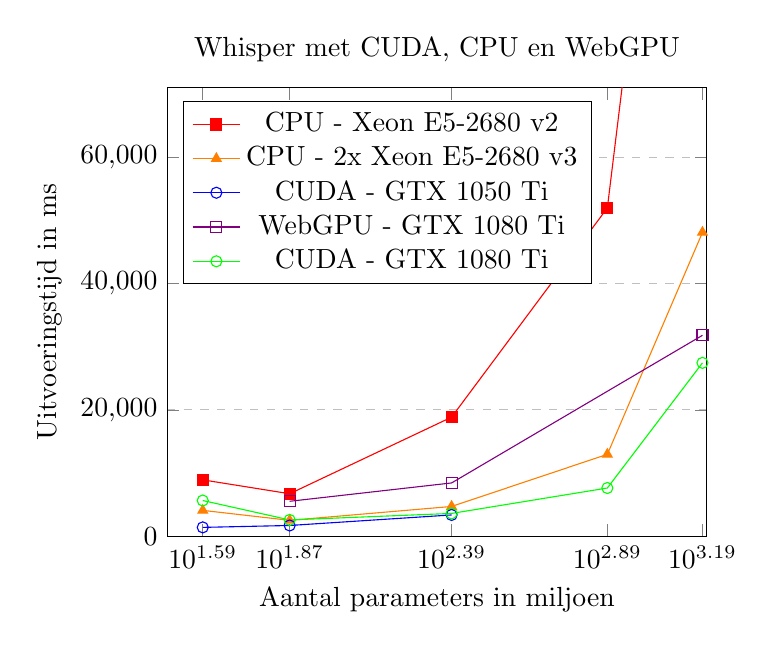
\begin{tikzpicture}
    \begin{semilogxaxis}[
        title={Whisper met CUDA, CPU en WebGPU},
        xlabel={Aantal parameters in miljoen},
        ylabel={Uitvoeringstijd in ms},
        xmin=30, xmax=1600,
        ymin=0, ymax=71000,
        xtick={39, 74, 244, 769, 1550},
        legend pos=north west,
        ymajorgrids=true,
        grid style=dashed,
        yticklabel style={
            /pgf/number format/fixed,
        },
        scaled y ticks=false
    ]
    \addplot[
            color=red,
            mark=square*
        ]
        coordinates {(39,8919)(74,6721)(244,18849)(769,51980)(1550,175378)};
        \addlegendentry{CPU - Xeon E5-2680 v2}

    \addplot[
        color=orange,
        mark=triangle*
        ]
        coordinates {(39,4088)(74,2508)(244,4706)(769,12963)(1550,48107)};
        \addlegendentry{CPU - 2x Xeon E5-2680 v3}

    \addplot[
            color=blue,
            mark=o
        ]
        coordinates {(39,1393)(74,1694)(244,3362)};
        \addlegendentry{CUDA - GTX 1050 Ti}
    
    \addplot[
            color=violet,
            mark=square
        ]
        coordinates {(74,5526)(244,8431)(1550,31814)};
        \addlegendentry{WebGPU - GTX 1080 Ti}

    \addplot[
            color=green,
            mark=o
        ]
        coordinates {(39,5647)(74,2574)(244,3602)(769,7629)(1550,27448)};
        \addlegendentry{CUDA - GTX 1080 Ti}
    \end{semilogxaxis}
\end{tikzpicture}

\section{Conclusies}

\textit{WebGPU} biedt aanzienlijke voordelen voor \textit{AI}-modellen in webapplicaties, met hoge prestaties en verbeterde privacy. Het ontgrendelt rekenkracht vergelijkbaar met traditionele \textit{low-level API}'s, waardoor zowel inferentie als training van \textit{AI}-modellen in de browser mogelijk is.

\textit{WebGPU} vermindert de noodzaak voor externe diensten, verlaagt kosten, en beschermt de privacy van eindgebruikers. De technology is reeds beschikbaar voor 70\% van de internetgebruikers en kan hierdoor op grote schaal ingezet worden.

Hoewel nog in ontwikkeling, tonen nieuwe implementaties indrukwekkende resultaten, waardoor \textit{WebGPU} aantrekkelijk is voor kleinschalige softwareoplossingen. Het maakt \textit{AI} toegankelijker, met verbeterde privacy en minder afhankelijkheid van externe diensten. Hierdoor is \textit{WebGPU} een aantrekkelijke keuze voor bedrijven en ontwikkelaars die willen profiteren van \textit{AI} zonder de nadelen van complexe technologieën en privacyrisico's. Een gebruiksvriendelijke implementatie van \textit{large language models} ondersteund door \textit{WebGPU} kan worden uitgetest op \href{https://chatgpu.qwict.com}{chatgpu.qwict.com}. Hiervoor is een browser vereist die \textit{WebGPU} ondersteunt.

\section{Toekomstig onderzoek}

Toekomstig onderzoek over de privacy- en cyberveiligheidsaspecten van \textit{WebGPU} is nog vereist, waaronder de impact op digital \textit{fingerprinting} en gevoeligheid voor \textit{side-channel} aanvallen.

Daarnaast is het belangrijk om te onderzoeken hoe de technologische capaciteiten van eindgebruikersapparaten de prestaties van \textit{AI}-modellen beïnvloeden. Browserfabrikanten en webontwikkelaars moeten verder werken aan het optimaliseren van \textit{WebGPU} zodat een breed scala aan apparaten de volledige potentie van deze technologie kunnen benutten.

\end{multicols}
\end{document}